\documentclass{article}
\usepackage{note_preamble}

\usepackage{titling}
\setlength{\droptitle}{-2cm}


\lstset{style=python-style1}

\begin{document}
\title{Machine Learning Notes}
\author{Zach Virgilio}
\maketitle 

\section*{Makemore notes}
\subsection*{Diagnostic Tools and Visualization}
    \begin{enumerate}
        \item Activation saturation of non-linear layers, i.e. $\tanh$ or ReLu etc.  For $\tanh$ layers, want to make sure the distribution is fairly even, and not tailed towards $\pm 1$ like in:

        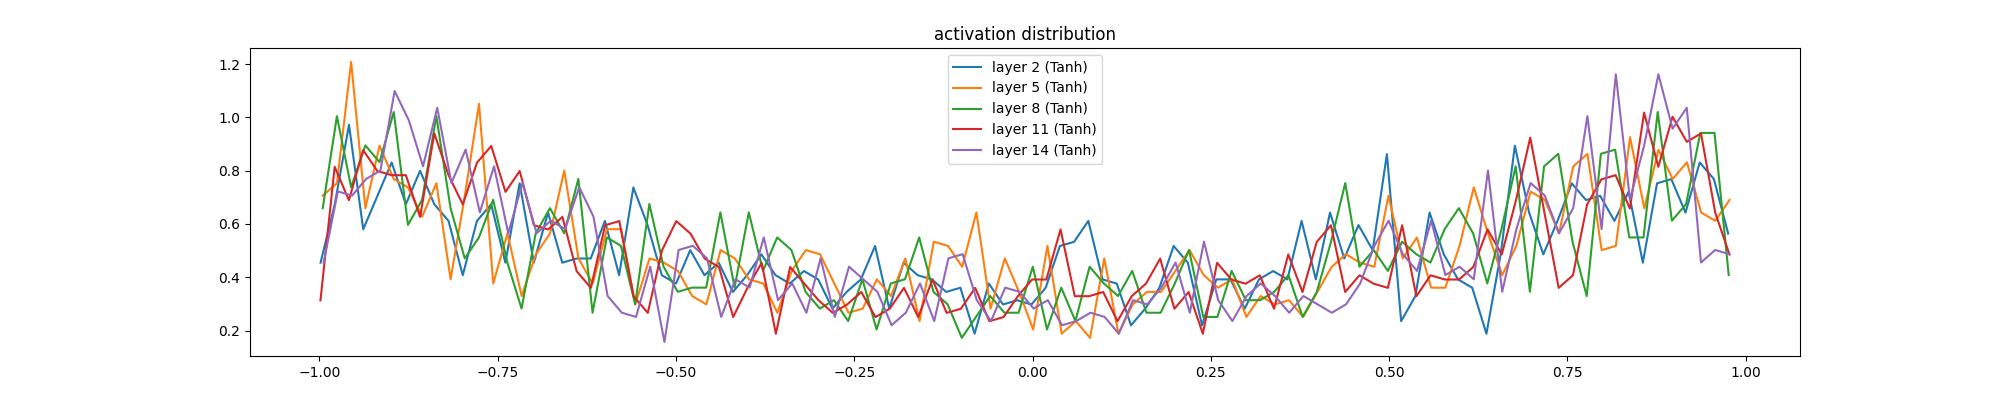
\includegraphics[width=0.9\textwidth]{images/tanh-activation}        

        Produced with \ref{code:activation-graph}.  
        This is important, because neurons with activations of $\pm 1$ will have gradients of $0$, as $\frac{d}{dx}\tanh x = 1 - (\tanh x)^2$, leading to dead neurons which don't learn. 
        The same phenomena occurs for sigmoid non-linearity.
        These are forward pass statistics

        \item Gradients of the non-linear layers.  For $\tanh$ they can look like:

        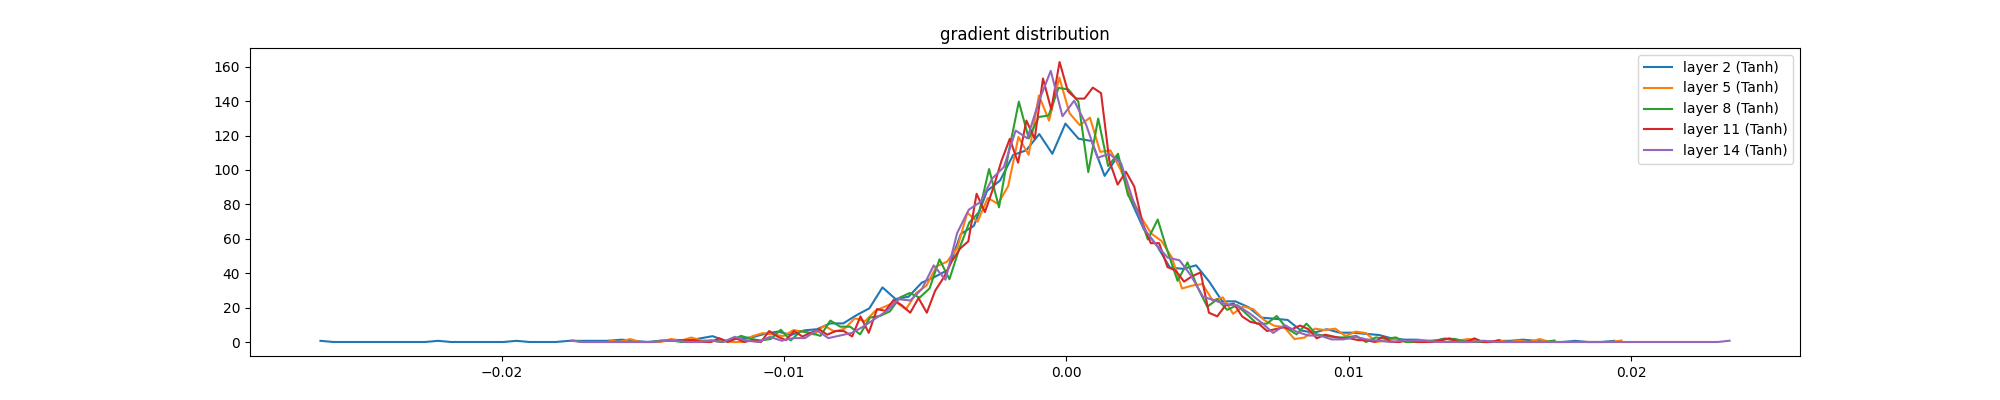
\includegraphics[width=0.9\textwidth]{images/dsitribution of gradients.png}

        Produced with \ref{code:grad-graph}.  These are backward pass statistics since they involve the gradient

        \item The ratio between the gradient and the parameter.  
        Should be similar for each layer after the first and before the last.  
        Restricting to 2-dim parameters, i.e. weights of the linear layers, not biases or $\gamma$ and $\beta$ in batch norm.

        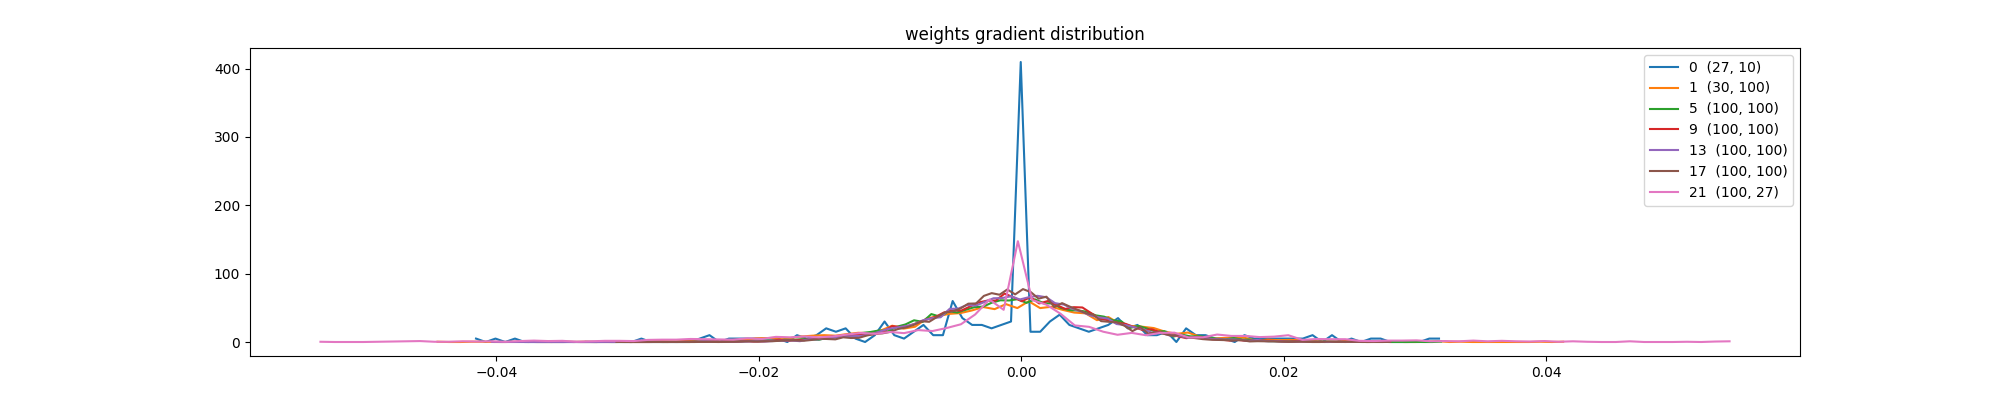
\includegraphics[width=0.9\textwidth]{images/grad-ratio.png}

        Produced with \ref{code:grad-scale-graph}.

        \item The size of the updates relative to the parameters.  
        As an estimate, want the $\log_{10}$ to be around $10^{-3}$. 
        This can be more informative than the gradient to data ratio, since what matters in learning is the size of the update.

        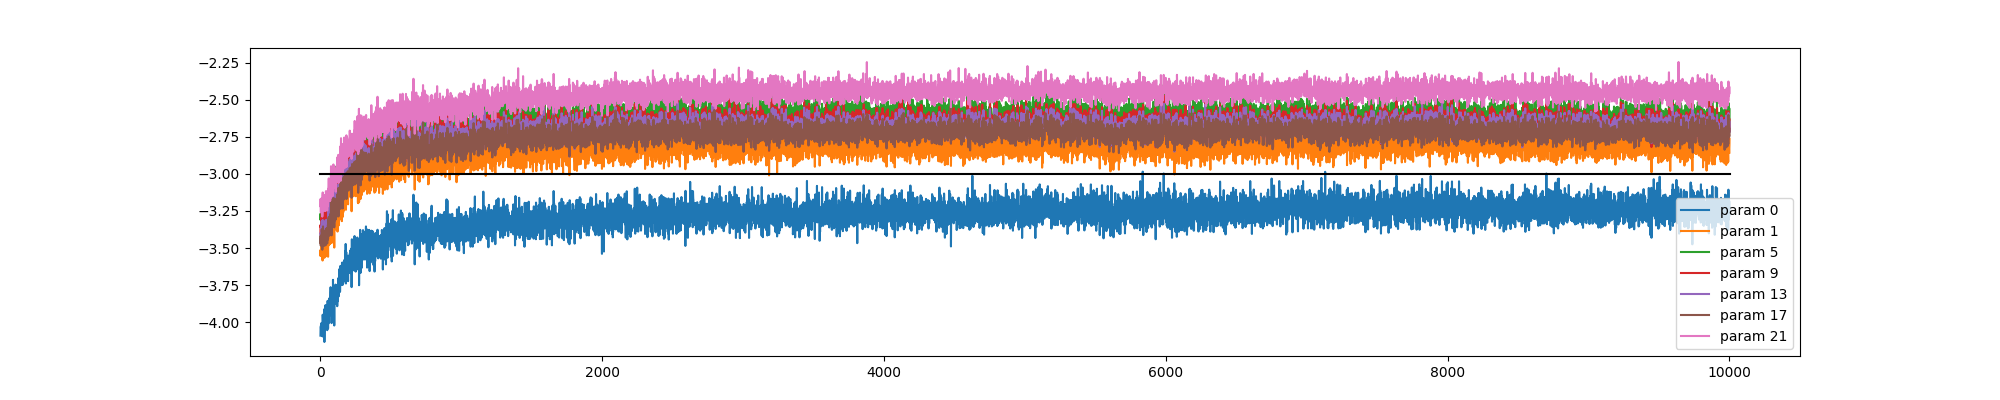
\includegraphics[width=0.9\textwidth]{images/update-ratio.png}

        Produced with \ref{code:update-graph}.
    \end{enumerate}

\begin{redbox}{Question}
    Why do we look at the ratio of grad standard deviations to parameter standard deviation (similarly for updates), instead of absolute values.
\end{redbox}

\subsection*{Batch Normalization}
Batch normalization is a technique used to stabilize training.  
It computes the mean and sd of the batch and uses that to normalize the batch to a standard normal distribution.  
This helps ensure neuron activation is more stable.
For example, if the non-linear layer is $\tanh$, it will take values of $\pm 1$ for inputs that are too far away from 0.  Oversaturation could keep some neurons always on or off.
It also means that adding a bias in a linear layer that comes before a batch normalization step is redundant as that bias is added to the norm and immediately subtracted, rendering it useless.


\subsection*{Backpropogation}
Be aware when a column is replicated before an elementwise operation is performed, you need to sum the gradients along the duplicated rows.
If a value $x$ feeds into to different paths, need to sum those gradients together.
Keep track to make sure torch broadcasting is properly backpropagated, this can be done by checking shape.

\subsection*{Containers}
Containers from PyTorch are ways of organizing layers into lists or dicts.  

\subsection*{Expiremental Harness}
When training takes longer and longer, need a way to test hyper-parameters such as learning rates and tune those without running the full training over and over.

\section*{Makemore Code Snippets}
\begin{lstlisting}[language=Python, caption={Activation graph with matplotlib}, label={code:activation-graph}]    
# visualize histograms of layer activation
plt.figure(figsize=(20, 4))
legends = []

for i, layer in enumerate(layers[:-1]): #exclude output layer
    if isinstance(layer, Tanh):
        t = layer.out 
        print('layer %d (%10s): mean %+.2f, std %.2f, saturated: %.2f%%' % (i, 
                layer.__class__.__name__, 
                t.mean(), t.std(), 
                (t.abs()>0.97).float().mean()*100))
        hy, hx = torch.histogram(t, density=True)
        plt.plot(hx[:-1].detach(), hy.detach())
        legends.append(f'layer {i} ({layer.__class__.__name__})')
plt.legend(legends)
plt.title('activation distribution')
# plt.show()
\end{lstlisting}

\begin{lstlisting}[language=Python, caption={Gradients of $\tanh$ layers with matplotlib}, label={code:grad-graph}]
    # histogram of gradients
plt.figure(figsize=(20, 4))
legends = []
for i, layer in enumerate(layers[:-1]): #exclude output layer
    if isinstance(layer, Tanh):
        t = layer.out.grad
        print('layer %d (%10s): mean %+.2f, std %e' % (i, 
                layer.__class__.__name__, 
                t.mean(), t.std()))
        hy, hx = torch.histogram(t, density=True)
        plt.plot(hx[:-1].detach(), hy.detach())
        legends.append(f'layer {i} ({layer.__class__.__name__})')
plt.legend(legends)
plt.title('gradient distribution')
\end{lstlisting}

\begin{lstlisting}[language=Python, caption={Scale between gradients and values of parameters}, label={code:grad-scale-graph}]
# parameter values visualization
# scale of gradient compared to actual values
plt.figure(figsize=(20, 4))
legends = []
for i, p in enumerate(parameters): #exclude output layer
    t = p.grad 
    if p.ndim == 2:
        print('weight %10s | mean %+f | std %e | grad:data ration %e' % (tuple(p.shape), 
                t.mean(), t.std(), t.std() / p.std() ))
        hy, hx = torch.histogram(t, density=True)
        plt.plot(hx[:-1].detach(), hy.detach())
        legends.append(f'{i}  {tuple(p.shape)}')
plt.legend(legends)
plt.title('weights gradient distribution')
\end{lstlisting}

\begin{lstlisting}[language=Python, caption={Size of update scaled by size of the parameter}, label={code:update-graph}]
#before training code
ud=[]
##### TRAINING #####
# in training loop
# lr is learning rate
# this tracks the log base 10
with torch.no_grad():
        ud.append([(lr*p.grad.std() / p.data.std()).log10().item() for p in parameters])
####################
# at each update, keep track of log of update size compated to data size
# these should be low or else we are over updating
# last layer can be large since that layer was ariticially compressed
plt.figure(figsize=(20,4))
legends = []
for i,p in enumerate(parameters):
    if p.ndim == 2:
        plt.plot([ud[j][i] for j in range(len(ud))])
        legends.append('param %d' % i)
plt.plot([0, len(ud)], [-3, -3], 'k') # ratios should be 1e-3
plt.legend(legends)
plt.show()
\end{lstlisting}
\end{document}